\chapter{\textbf{Introduction}}
\label{ch:intro}

Understanding the origin of the elements has been the primary goal of nuclear astrophysics since its conception. Through the work of Burbidge, Burbidge, Fowler, and Hoyle \cite{Burbidge1957}, it was established that the chemical elements observed in our solar system were synthesized through nuclear burning in stars. Indeed, all but the smallest elements in our observable universe (hydrogen through boron) are the ashes of stellar burning. Consequently, in the quest to discover the nature of the elemental origins, we must understand the nature of stellar processes. From birth to death, stars undergo nuclear reactions in their interiors. With sufficient temperatures, the reaction products themselves undergo subsequent nuclear reactions. An evolutionary stage is reached at which point the star either explodes or otherwise ejects its material outward. This nuclear-processed material is mixed together with the ashes from neighboring stars, forming new stars with new compositions and therefore new nucleosynthesis. One of the most complex evolutionary stages of a star is known as the asymptotic giant branch (AGB) phase, and stars that we currently observe on this phase are known as AGB stars. This thesis focuses on these complex nucleosynthesis processes in massive AGB stars, including s-process nucleosynthesis resulting from thermal pulses, as well as hot-bottom burning at the base of the convective hydrogen envelope. These stellar processes are investigated through laboratory nuclear reaction experiments here on earth. In particular, transfer reaction experiments are used in this thesis as a surrogate for the direct reactions occurring in the stellar processes. These experiments provide information on the nuclear structure of the nuclei involved in the key reactions, and therefore they constrain the reaction rates that are crucial to nucleosynthesis.

The present chapter will provide an overview of the nuclear astrophysics topics addressed in this thesis. Chapter \ref{ch:reactions} will introduce the mathematical formalism for quantifying nucleosynthesis with reaction rates, as well as the formalism for transfer reactions. Chapter \ref{ch:Rb} will address the rubidium overabundance observed in massive AGB stars, as a result of s-process nucleosynthesis. The measurement of the $^{86}\mathrm{Kr}(^{3}\mathrm{He},d)^{87}\mathrm{Rb}$ transfer reaction is proposed to enhance our understanding of the closed-N shell nucleus $^{87}$Rb and its involvement in the rubidium overabundance. Chapter \ref{ch:exp} will introduce the experimental techniques that were used in this thesis to successfully perform transfer reaction experiments. Chapter \ref{ch:DAQ} will introduce the work that was done implementing a new digital data acquisition system (DAQ) for the focal-plane detector package at the Enge Split-Pole Spectrograph, which will replace the current analog system for future transfer reaction experiments. Finally, Chapter \ref{ch:GC} will address the abundance patterns in globular cluster NGC 2419, which may have originated from hot-bottom burning in massive AGB stars. The anomalous Mg--K abundance pattern observed in NGC 2419 is investigated with the $^{39}\mathrm{K}(^{3}\mathrm{He},d)^{40}\mathrm{Ca}$ transfer reaction, and new constraints are placed on the key potassium-destroying reaction $^{39}\mathrm{K}(p,\gamma)^{40}\mathrm{Ca}$ from the first-ever resolution of the 154 keV resonance in $^{39}\mathrm{K}+p$, among the other resonances of astrophysical interest.

%--------------------------------------------------------------------------
%--------------------------------------------------------------------------
\section{Overview of Asymptotic Giant Branch Stars}
% Evolution on the H-R diagram (figure). Early (E-AGB) phase versus thermally-pulsing (TP-AGB) phase. The hydrogen and helium burning shells in the TP-AGB phase (with figure). S-Process occuring in the inter-shell region during and between thermal pulses. Hot-bottom burning occuring between the base of the convective hydrogen envelope and the hydrogen-burning shell.

Asymptotic giant branch (AGB) stars produce about half of all elements heavier than iron in our galaxy \cite{Busso1999}, and they are one of the leading candidates for the origin of abundance anomalies in globular clusters \cite{Prantzos2007}. An understanding of these stars therefore provides insight into the origin of the elements. The asymptotic giant branch refers to the evolutionary track that these stars follow on a typical Hertzsprung-Russell (HR) diagram, which asymptotically approaches that of the red giant branch. HR diagrams show the luminosity of a star as a function of its effective temperature. These properties are often cataloged for each star observed in a globular cluster, for example, and the current evolutionary phase of a star can be determined from its relative position on the diagram. A theoretical example of the evolutionary track of a $5 M_{\odot}$ star is represented on the HR diagram of Fig. \ref{fig:5M_Evolution}. Starting from the zero-age main sequence (ZAMS), where the star first begins to burn hydrogen, the evolutionary track passes through the sub-giant branch (SGB), the red-giant branch (RGB), the horizontal branch (HB), the early (E-) and thermally-pulsing (TP-) asymptotic giant branch (AGB) phases, and the post-AGB branch. It then undergoes planetary nebula (PN) formation, before eventually becoming a white dwarf. Each of these branches represents a unique evolutionary phase of the star, many of which are described in the figure at key transitional points. As mentioned above, this thesis focuses on AGB stars, the evolutionary track of which is highlighted in red in the figure.

\begin{figure}[t]
\centering
\begin{tikzpicture}[scale=1.0, every node/.style={transform shape}]
\coordinate (a) at (3,1.7);
\coordinate (b) at (4.14,3.52);
\node at (0,0) {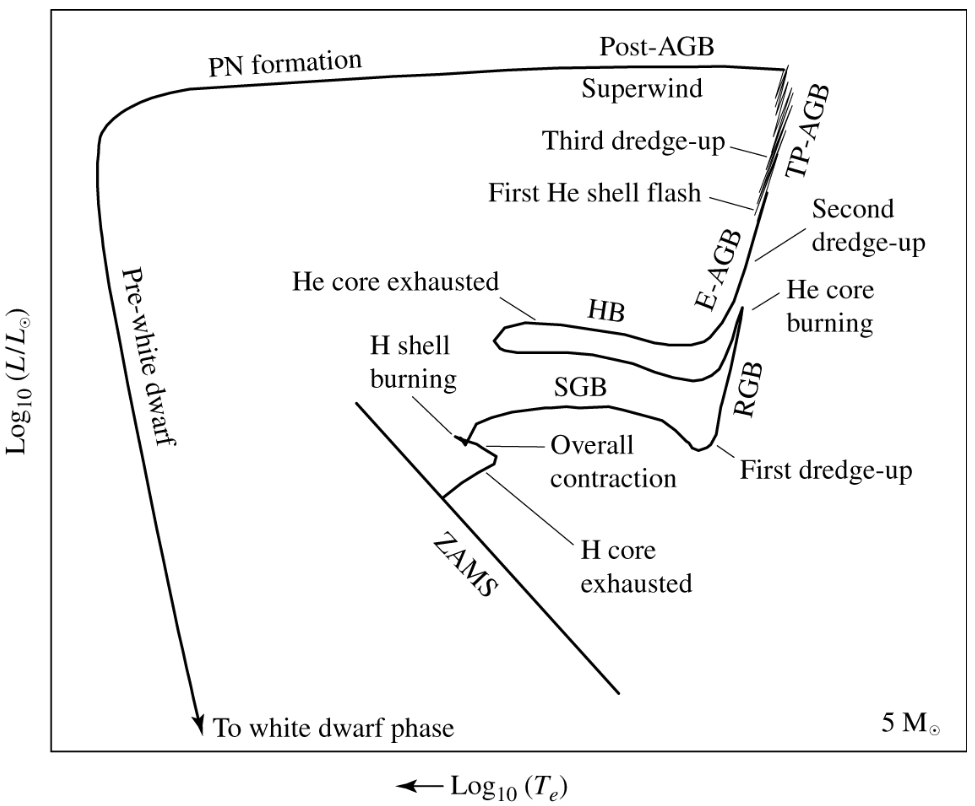
\includegraphics[width=5in]{Chapter-1/figs/5M_Evolution.png}};
\draw[rotate around={72:(a)},color=red] (a) ellipse (0.8 cm and 0.3 cm);
\draw[rotate around={72:(b)},color=red] (b) ellipse (0.8 cm and 0.3 cm);
\end{tikzpicture}
\caption{\label{fig:5M_Evolution}Evolution of a 5 $M_{\odot}$ star represented on the Hertzsprung-Russell (HR) diagram. The two-stages of the asymptotic giant branch (AGB) are highlighted in red. See text for definitions of acronyms. Figure adapted from Ref. \cite{Carroll2007}.}
\end{figure}

It is clear from Figure \ref{fig:5M_Evolution} that AGB stellar evolution is separated into two stages. The \emph{early-AGB} (e-AGB) stage occurs after both hydrogen and helium have been exhausted in the core of a star, leaving behind mostly inert carbon and oxygen. Hydrogen and helium burning is still active in separate shells around the core, with a helium-rich intershell region in between. The far more active hydrogen-burning shell perpetually increases the density and temperature of the intershell region, until the rate of energy generated by the helium-burning shell is greater than the rate at which energy can be transported outward through radiative diffusion \cite{Iliadis2015}. A thermal instability, called a \emph{thermal pulse}, occurs as a result, initiating the \emph{thermally pulsing AGB} (TP-AGB) stage, shown in Figure \ref{fig:AGB_Structure}. This pulse causes the helium-burning shell to extend into the intershell region and ignite the hydrogen-burning shell, rendering it inactive for a brief period. The nuclei inside the intershell region get carried outward through the convective hydrogen envelope toward the surface of the star, where they are ejected by stellar winds. The hydrogen-burning shell takes over once again as the dominant energy-producer after the thermal pulse, and this cycle repeats for on the order of tens to hundreds of pulses \cite{Habing2004}.

%\begin{figure}[t]
%\centering
%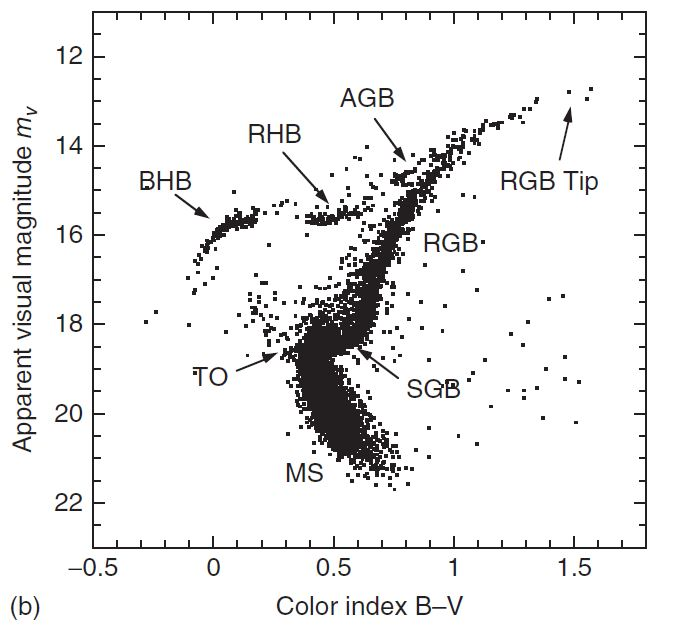
\includegraphics[width=5in]{Chapter-1/figs/HRDiagram.jpg}
%\caption{\label{fig:HRDiagram}The Hertzsprung-Russell (HR) diagram. Figure adapted from Ref. \cite{Iliadis2015}.}
%\end{figure}

\begin{figure}[t]
\centering
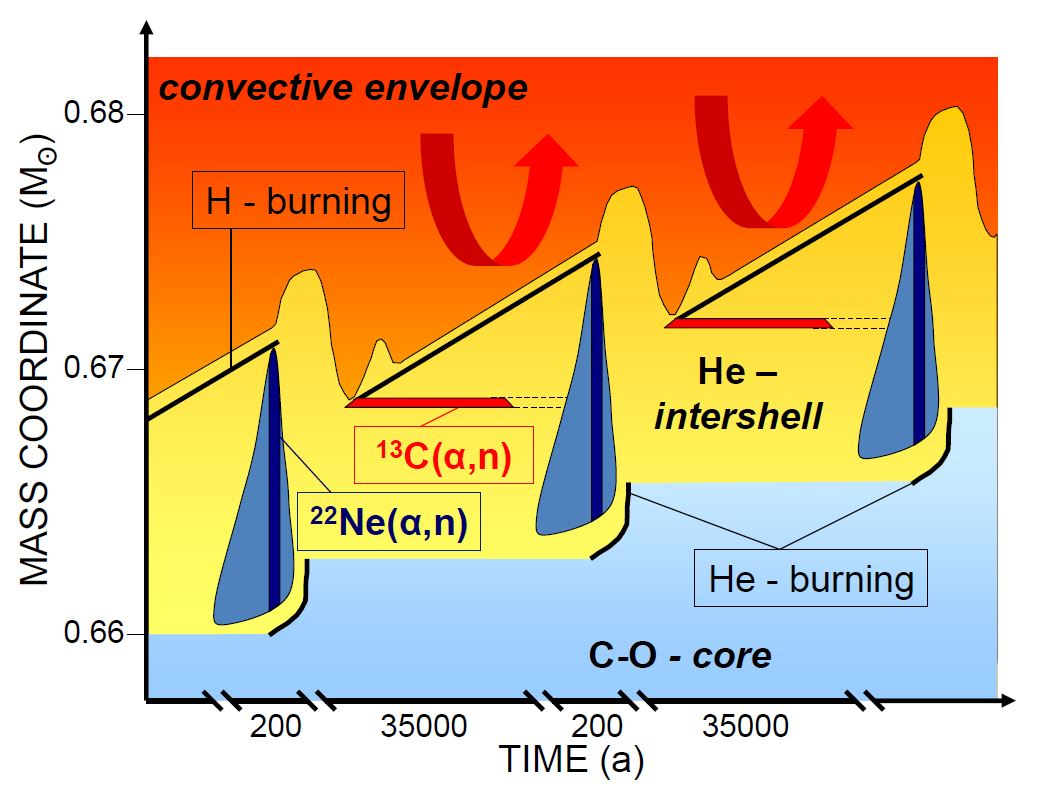
\includegraphics[width=6.5in]{Chapter-1/figs/sProcess_AGB.JPG}
\caption{\label{fig:AGB_Structure}The evolution and structure of a thermally pulsing AGB star. Three thermal pulses are depicted in blue, extinguishing the hydrogen burning shell. The neutron sources $^{13}\mathrm{C}(\alpha,n)^{16}\mathrm{O}$ and $^{22}\mathrm{Ne}(\alpha,n)^{25}\mathrm{Mg}$ are shown to be active between pulses and during pulses, respectively. Figure adapted from Ref. \cite{Reifarth2014}.}
\end{figure}

Both during thermal pulses and during the interpulse period, the helium-rich intershell region produces a large flux of neutrons. These neutrons originate from the neutron sources, $^{13}\mathrm{C}(\alpha,n)^{16}\mathrm{O}$ and $^{22}\mathrm{Ne}(\alpha,n)^{25}\mathrm{Mg}$. The former reaction is the dominant neutron source during the interpulse period, where temperatures are between $100$ MK $\lesssim T \lesssim$ 300 MK and neutron densities are roughly $N_{n} \approx 10^{7}$ $\mathrm{cm}^{-3}$. During thermal pulses, where $T$ and $N_{n}$ increase, the latter reaction is dominant and occurs at $T \gtrsim 300$ MK and $N_{n} \approx 10^{10}$ $\mathrm{cm}^{-3}$. Nucleosynthesis occurs in the intershell region via a series of neutron captures and beta decays, known as the s-process, described in Section \ref{sec:s-process}.

In the case of intermediate-mass or massive AGB stars ($M \gtrsim 4 \, M_{\odot}$), the convective hydrogen envelope reaches down to the top of the hydrogen-burning shell during the interpulse period, where temperatures are at least 50 MK. The resulting hydrogen burning nucleosynthesis is called \emph{hot-bottom burning}, detailed in Section \ref{sec:hot-bottom-burning}, and the products of this burning are brought to the surface by the convective hydrogen envelope.

%--------------------------------------------------------------------------
%--------------------------------------------------------------------------
\section{s-Process Nucleosynthesis} \label{sec:s-process}
% Main and weak components of the s-process here
% s-process paths picture

% Both during thermal pulses and during the interpulse period, the helium-rich intershell region produces a large flux of neutrons. These neutrons originate from the neutron sources, $^{13}\mathrm{C}(\alpha,n)^{16}\mathrm{O}$ and $^{22}\mathrm{Ne}(\alpha,n)^{25}\mathrm{Mg}$. The former reaction is the dominant neutron source during the interpulse period, where temperatures are between about $100$ MK $\lesssim T \lesssim$ 300 MK and neutron densities are roughly $N_{n} \approx 10^{7}$ $\mathrm{cm}^{-3}$. During thermal pulses, where $T$ and $N_{n}$ increase, the latter reaction is dominant and occurs at $T \gtrsim 300$ MK and $N_{n} \approx 10^{10}$ $\mathrm{cm}^{-3}$. Nucleosynthesis occurs in the intershell region via a series of neutron captures and beta decays, known as the s-process, described in Section \ref{sec:s-process}.

% Neutrons lead to nucleosynthesis for A>60

Most light nuclei below the iron-peak at mass number $A \approx 60$ are formed through charged-particle fusion reactions in stars, where temperatures are sufficient for transmission through the repulsive Coulomb barrier via quantum tunneling. The synthesis of nuclei heavier than the iron-peak, however, cannot be explained by these charged-particle fusion reactions. At low temperatures, the transmission probability through the large Coulomb barrier of heavy nuclei becomes prohibitively small, while at high temperatures, nuclear statistical equilibrium favors the production of iron-peak nuclei due to their large binding energy per nucleon. Nuclei with $A \gtrsim 60$ must be formed instead by neutron capture, where Coulomb repulsion is no longer a factor. Neutron capture will generate neutron-rich isotopes of a given element, some of which eventually undergo $\beta$--decay if they are unstable. The daughter nuclei will then capture neutrons until another unstable isotope is reached, and the process continues this way up to some of the heaviest nuclei.

%--------------------------------------------------------------------------
% s-process vs r-process

When the neutron density in the astrophysical environment is sufficiently small such that unstable nuclei preferentially $\beta$--decay, the ensuing nucleosynthesis is referred to as the \emph{s-process}. This is a relatively slow process (hence the \emph{s-}), as the nucleosynthesis can only proceed based on the half-lives of the unstable nuclei. If, on the other hand, the neutron density is sufficiently large such that unstable nuclei preferentially neutron-capture, the ensuing nucleosynthesis is referred to as the \emph{r-process} because this happens at a much more (\emph{r-})apid pace. These two processes occur in different astrophysical sites and are equally responsible for almost all of the heavy nuclei in the observable universe. Some heavy nuclei are referred to as s-only or r-only nuclei because only one of these processes accounts for their abundance. The focus of Chapter \ref{ch:Rb} will be on s-process nucleosynthesis, as this occurs in AGB stars both during thermal pulses and during the interpulse period.

%--------------------------------------------------------------------------
% s-process path and abundance evolution

To illustrate how the s-process works, consider the chain of reactions shown in Figure \ref{fig:sProcess_path}, starting with the most abundant stable nucleus formed at the end of the stellar fusion reaction chains, $^{56}$Fe. This is referred to as a \emph{seed nucleus} because it is the nucleus that initiates the s-process reaction chain. Stable nuclei are shown in black in the figure, nuclei unstable to $\beta^{-}$--decay are shown in blue, and nuclei unstable to $\beta^{+}$--decay or electron capture (EC) are shown in red. As is typical of a chart of the nuclides, neutron number increases to the right and proton number increases upward. Neutron-capture is therefore represented by an arrow to the right, while $\beta$--decays and electron capture are represented by diagonal arrows due to the conversion of a neutron to a proton, or vice versa. If there is a sufficient neutron density $N_{n}$ in the astrophysical environment, the neutron-capture of $^{56}$Fe, $^{56}\mathrm{Fe}(n,\gamma)^{57}\mathrm{Fe}$, leads to the stable nucleus $^{57}$Fe. The two subsequent neutron-captures,  $^{57}\mathrm{Fe}(n,\gamma)^{58}\mathrm{Fe}$ and  $^{58}\mathrm{Fe}(n,\gamma)^{59}\mathrm{Fe}$, on the stable $^{57}$Fe and $^{58}$Fe nuclei, respectively, leads to the unstable $^{59}$Fe nucleus. The nucleosynthesis path has now lead to an \emph{s-process branching}, and $^{59}$Fe is referred to as a \emph{branching point nucleus}. At these branchings, the decay constant for $\beta$--decay, $\lambda_{\beta}$, is approximately equal to the decay constant for neutron capture, $\lambda_{n\gamma}$. That is, $\lambda_{\beta} \approx \lambda_{n\gamma}$, and the path splits into two branches with approximately equal probability. These branchings are sensitive to neutron density $N_{n}$ and the neutron-capture cross section $\sigma_{n\gamma}$ of the unstable branching point nucleus, described below. After the s-process branching, the path continues in this way up to some of the heaviest nuclei.

\begin{figure}[t]
\centering
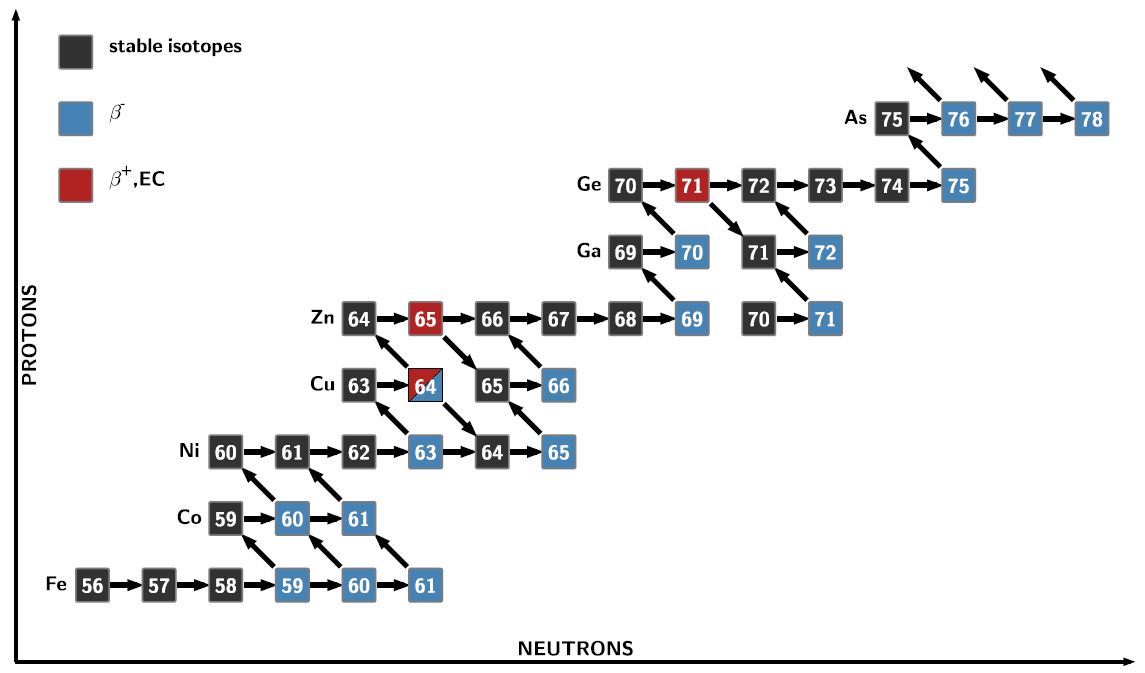
\includegraphics[width=6.5in]{Chapter-1/figs/sProcess_path.jpg}
\caption{\label{fig:sProcess_path}The s-process path from iron to arsenic. The stable nuclei in black undergo neutron capture, while the unstable nuclei in blue ($\beta^{-}$-decay) and red ($\beta^{+}$-decay or electron capture) either decay or undergo neutron-capture depending on their half-lives and the neutron density $N_{n}$. At s-process branchings, e.g. $^{59}$Fe, the probability for neutron-capture and decaying is approximately equal, hence the path is split into two branches. Figure adapted from Ref. \cite{Reifarth2014}.}
\end{figure}

% "Classical" s-process (Eqns. 5.173 - 5.192 in Nuclear Physics of Stars). Disregards time dependence of s-process parameters, such as neutron density and stellar temperature. Makes no assumption on the stellar site or specific reactions acting as neutron sources. The classical model offers remarkable insight into the s-process regardless. It explains the main, weak, and strong s-process components. Eqn. 5.192 describes the simplest case of an s-process branching, but each branching is different. 

% Include custom simple neutron capture and beta decay figure with a branching.
% Include figure of overall Reifarth s-process path.
% For math, maybe only include 2 sets of equations - 5.173 to 5.174 and 5.191 (excluding the tau part) to 5.192 (excluding the top line) --- Don't need Tau for any of these!

% Use Nuclear Physics of Stars Figure 5.68 parts (b) and (c) with the math. Part (b) assumes radioactive nuclei always undergo beta-decay. Can start from Eqn. 5.173, even removing part (a).



%--------------------------------------------------------------------------
% weak-component vs main-component (vs strong-component?) in the s-process 

% Different sites (AGB, massive star), weak is for 60 < A < 90, main is 90 < A < 205, strong A > 205
% Treated separately, they describe all s-only nuclide abundances

%--------------------------------------------------------------------------
%--------------------------------------------------------------------------
\subsection{Rubidium Overabundance} \label{subsec:Rb_Overabundance}

% "Rb problem"
% 86Rb branch, 87Rb abundance - connected to 22Ne(a,n)25Mg reaction

%--------------------------------------------------------------------------
%--------------------------------------------------------------------------
\section{Hot-Bottom Burning} \label{sec:hot-bottom-burning}

%In the case of massive AGB stars ($M \gtrsim 4 M_{\odot}$), the convective hydrogen envelope reaches down to the top of the hydrogen-burning shell during the interpulse period, where temperatures are at least 50 MK. The resulting hydrogen burning nucleosynthesis is called \emph{hot-bottom burning}

%--------------------------------------------------------------------------
%--------------------------------------------------------------------------
\subsection{Candidate for Globular Cluster Abundance Anomalies} \label{subsec:GC_Candidate}

% AGB stars for Prantzos 2007 and Ventura 2012, Super-AGB stars for Illiadis 2016